In this section an overview of the logic and the components which compose the system are introduced since they are explain in detail in the following sections. 

Basically, the platform has been design in a modular way and it is composed of the State manager, the vision, motion and input/output modules that interact with the different sensors, actuators and boards as it is shown in figure \ref{fig:components}.

\begin{figure}[h!]
\centering
	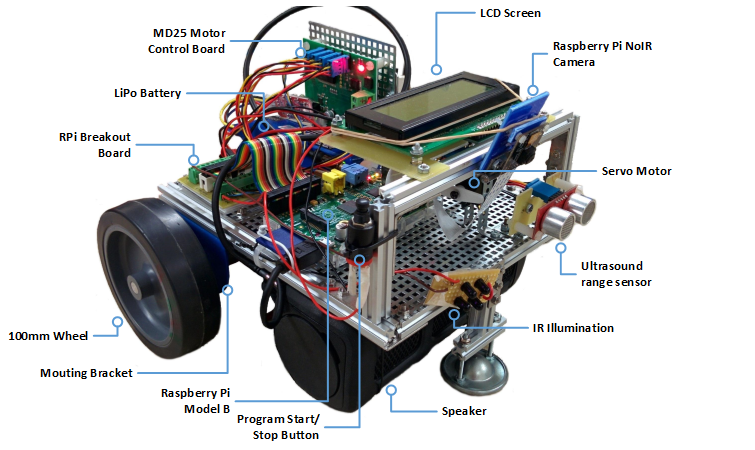
\includegraphics[width=0.8\textwidth]{robot.png}
	\caption{Overview of the robot's components}
	\label{fig:components}
\end{figure}

The sensors provided are an ultrasonic proximity sensor, a Pi nearly infrared camera and a start/stop button. This camera needs some source of infrared light thus four infrared LEDs are located in the front of the the robot. Additionally, it uses an LCD display located on the top to provide visual feedback of the current state as well as a speaker located under the robot for a sound feedback.

\newpage
The most important actuators are the motors located at both sides of the platform controlled by a MD25 motor control board as well as the servomotor that if it is necessary, can be configured in order to control the angle of vision of the NIR camera.

Moving to the logic part (figure \ref{fig:overview}), the state manager sets the current state of the robot according to the proximity sensor but mainly based on the information coming from the vision module which directly interacts with the PiCamera. The vision module carries out the analysis of the images being able to segment the scene and extract the position of the sings on the floor. It strongly uses the OpenCV library to perform this task running on the Raspberry Pi. 

\begin{figure}[h!]
     \centering
     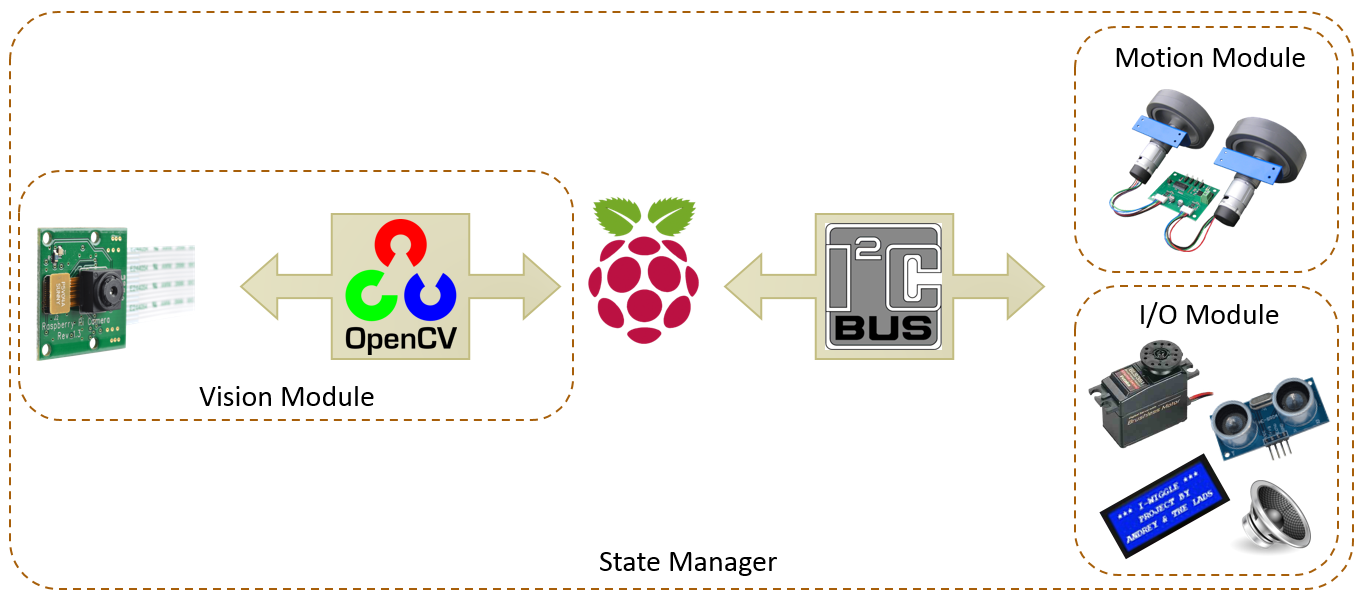
\includegraphics[width=0.7\textwidth]{overview.png}
     \caption{System overview}
     \label{fig:overview}
\end{figure}

Once a sign is detected, for instance, the state manager switches the current state acting over the motion module which controls the two motors providing the proper angular and linear speeds. The way both, the motion and the input/output module interact with the board is through the $I^2C$ bus enabled in Raspberry Pi.

On the other hand, the input/output module as its name describes, provides visual and sound feedback to the current state of the system enhancing the communication with the user.
